\documentclass[10pt]{beamer}
\usetheme[progressbar=frametitle]{metropolis}
\setbeamercovered{transparent}
\usepackage{appendixnumberbeamer}
\usepackage{booktabs}
\usepackage[scale=2]{ccicons}
\usepackage{pgfplots}
\usepackage{amssymb}
\usepackage{xspace}
\usepackage{mathtools}
\usepackage{graphicx}
\usepackage{subcaption}
\usepgfplotslibrary{dateplot}
\newcommand{\themename}{\textbf{\textsc{metropolis}}\xspace}
\usepackage[
backend=biber,
style=bwl-FU,
citestyle=bwl-FU
]{biblatex}
\addbibresource{bibliography.bib}
\geometry{paperwidth=180mm,paperheight=105mm}
\title{Regression Trees}
\author{Timothy Currie}
\institute{Universität Bonn}
\date{\vspace{2cm} \textbf{\large{Wissenschaftliches Arbeiten}} \\ \textbf{25/06/2024} \\ 
       \vspace{1cm} \textbf{Supervisor:} Dr. Elias Wolf \\ 
       \textbf{Matrikelnummer:} 50074426}
\begin{document}
\maketitle













\begin{frame}{Simulation: Linear Data}
    \begin{columns}[T]
        \begin{column}{0.5\textwidth}
        \begin{figure}
            \centering
            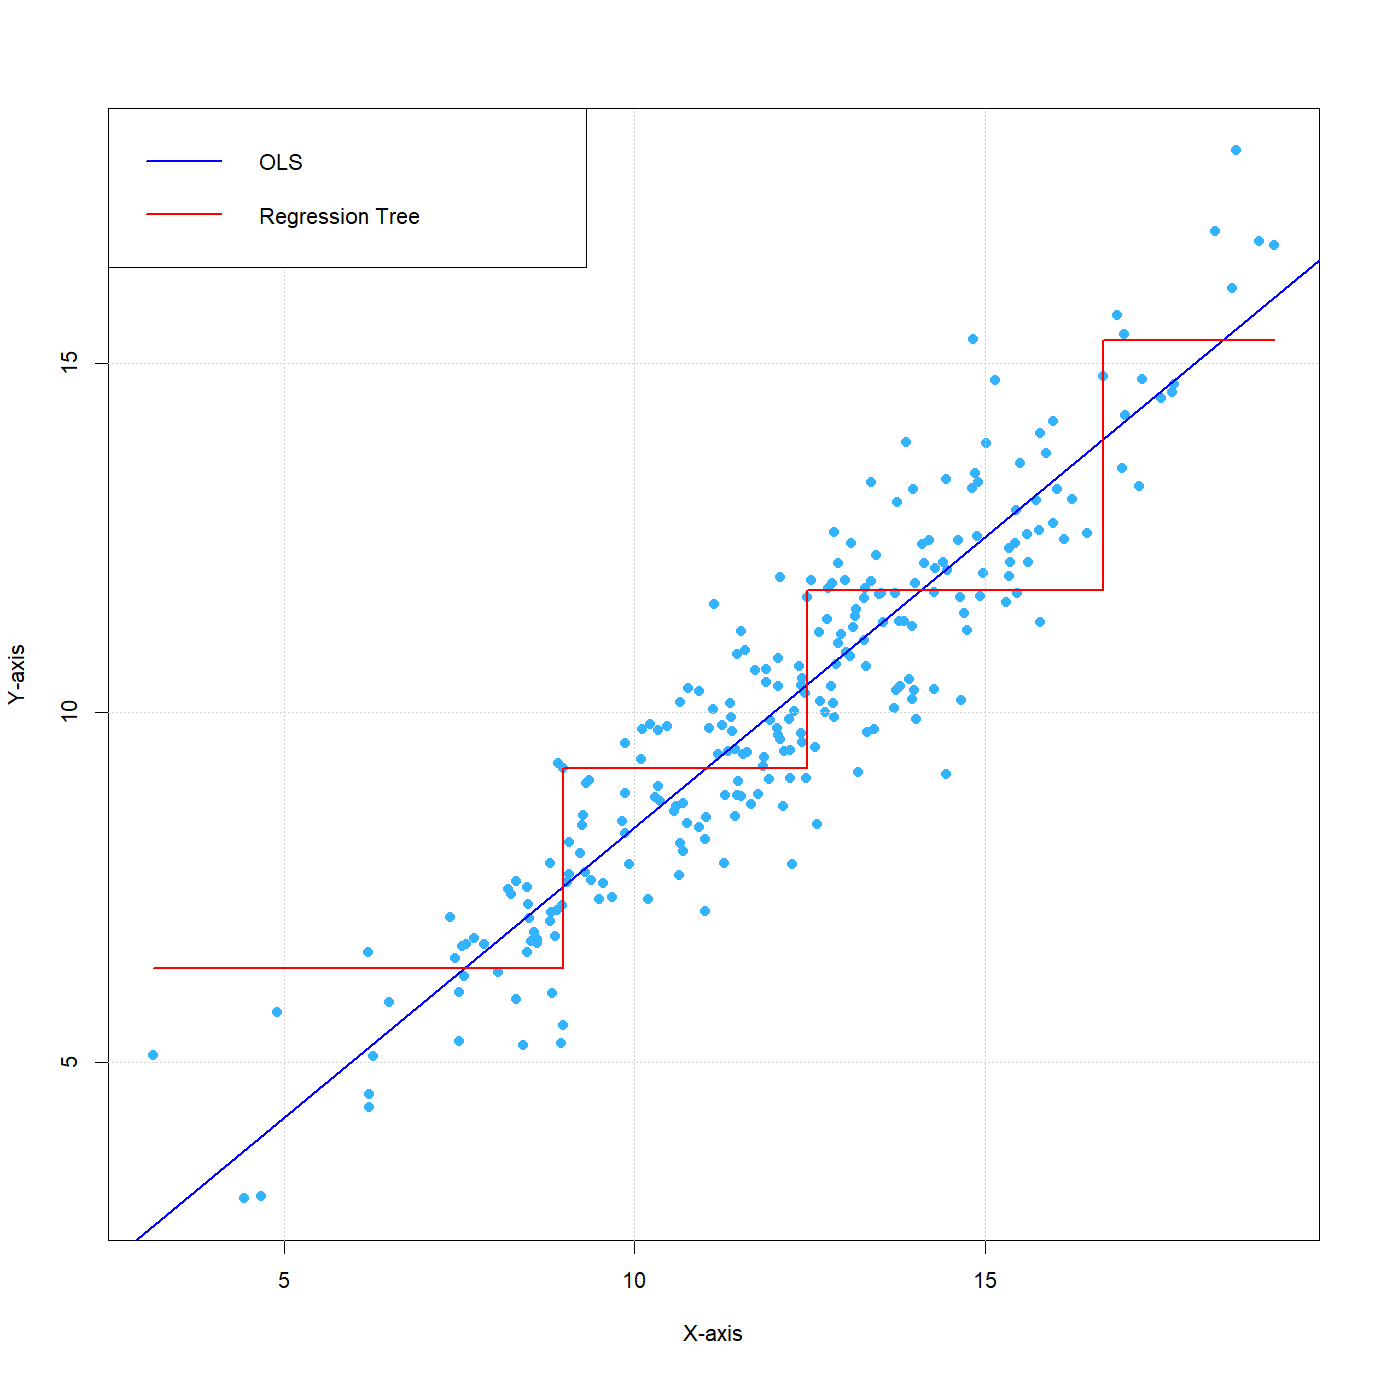
\includegraphics[width=1\linewidth]{OLS vs Tree.png}
            \caption{Linear Relation between Variables}
            \label{fig:sub4}  % Changed label to be unique
            \end{figure}
        \end{column}
        \begin{column}{0.5\textwidth}
        
            \begin{itemize}
                        \vspace{0.7cm}

            \item We will run all simulations 400 times.
                 \item For now the regression trees will have 4 terminal Nodes.
                \item And we will always compare the Mean Squared Error (MSE).
                \vspace{1cm}
                \item \textbf{Results:}
                \item \textbf{MSE} for OLS model: \textbf{0.9917} 
                \item \textbf{MSE} for regression tree model: \textbf{1.4935} 
            \end{itemize}
        \end{column}
    \end{columns}
\end{frame}





\end{document}